\documentclass[pre,twocolumn,superscriptaddress,nofootinbib]{revtex4-2}
\usepackage{graphicx}
\usepackage{amsmath}
\usepackage{booktabs}
\usepackage[hidelinks]{hyperref}

\begin{document}

\title{The curled torus burps: front-driven decompactification between ordered states in a graph model of
emergent geometry}

\author{Emily Smith}
\email{emilysmithcreate@gmail.com}
\affiliation{Independent researcher, Charlottesville, Virginia, USA}

\date{Corrected version, 25 September 2026}

\begin{abstract}
In combinatorial quantum gravity (CQG) the energy of a four-regular bipartite graph is built from its total
Ollivier curvature, which splits into a global term that rewards squares and a local term that removes the reward
for a third square on an edge. We study the family of graph energies obtained by multiplying the local
term by a coefficient $\lambda$. Only $\lambda = 1$ is CQG; for $\lambda \ne 1$ the energy is no longer a
curvature, and every result below is at $\lambda > 1$, in this neighbouring family and not in CQG itself.
For $\lambda \ge 1$ the flat lattice torus is a ground state exactly, and a $4 \times L$ torus, one direction curled to a single square, lies
$4(\lambda - 1)$ per vertex above it. At $\lambda = 1.25$ the curled torus is metastable. Under the local
edge-switch dynamics used to sample the model, with Metropolis acceptance, the minimum energetic barrier to leave
it is a single move, $\Delta E^\ddagger = 12$, offered at a rate we count exactly, so the mean waiting time follows
an Arrhenius law with nothing fitted, and the wait is close to memoryless (the pre-registered checks pass in most
cells and fail in some, on a band too tight for the sample, on rare very long waits, or on a wide spread of waits;
Sec.~\ref{sec:lambda}). After the first exit the conversion spreads as a
single front: at half conversion 98.8 to 99.8\% of vertices belong to one ordered state or the other, and the
energy released is exactly $\varepsilon = 4(\lambda-1)$ per vertex. Under an energy-conserving version of the
same dynamics, a seed equal to the barrier, 12 units, sets off the change at every size from 48 to 192
vertices and nothing smaller does, while the release grows with the system. The change then completes only if
the reservoir can absorb the release, and it leaves about one relic defect of fixed size at every size tested,
from 64 to 288 vertices. Mapped from $\lambda = 1.05$ to 1.45 in three pre-registered runs, each inconclusive
by the letter of its rules, the torus is metastable up to 1.35; the change keeps its two-order, single-front
character from 1.05 to 1.30 in all three runs and begins to break up at 1.35, finishing cleanly near
$\lambda = 1$ and leaving more defects as $\lambda$ grows. The release vanishes at $\lambda = 1$, the CQG value.
The Arrhenius test and the seed threshold were exploratory; every verdict quoted was pre-registered, and the
two-state verdict at $\lambda = 1.25$ was reached after amendments to its energy gate, three of them written after
the data they judged.
\end{abstract}

\maketitle

\section{Introduction}

In combinatorial quantum gravity (CQG) \cite{T17,KTB19,T25} geometry emerges from random graphs driven by
a discrete Ricci curvature. The question studied so far is whether geometry forms out of the random phase
sharply or smoothly: a first-order transition with hysteresis when only the global term is kept
\cite{GV21}, a continuous one with the full action \cite{KTB19,T25}. A different kind of
change has not, as far as we have found, been studied in this model: one \emph{ordered} arrangement
turning into another. Such changes matter for the proposal that dark matter consists of long-lived
regions of the graph stuck in a different discrete arrangement \cite{T24}. We study the simplest such
change we have found, a torus with one direction curled, opening into the flat torus. It exists as a
metastable state only when the local term is weighted by a coefficient $\lambda > 1$, where the energy is no
longer the total curvature; this is therefore a study next to CQG, not in it, and the curled torus is not an
allotrope in the sense of Ref.~\cite{T24}. It is a decompactification in
miniature: a curled direction opens to full size, and the local dimension defined below rises from 1 to 2.
Because the change waits quietly and then releases a fixed amount of energy all at once, we call the whole
event a burp. We map it along $\lambda$, down to $\lambda = 1.05$, and follow its decay.

Why deform CQG at all? At $\lambda = 1$ an edge carrying three squares costs exactly what an edge carrying two
costs, so the flat torus, the curled torus and the 4-cube are degenerate, and no ordered arrangement can turn
into another with any release. The coefficient $\lambda$ lifts that degeneracy and changes nothing else: the
states, the moves and the hard-core rule are those of CQG. For $\lambda > 1$ the ground states are the arrangements with two
squares on every edge, the flat torus and its twisted relatives, and each curled direction costs a known energy
per vertex. The family is therefore a controlled
laboratory for a change between two ordered arrangements, in which the barrier, the release and the relic can
each be counted exactly, and $\lambda \to 1$ connects it to CQG.

Every kinetic statement below, about waiting times, barriers and fronts, concerns one Markov chain: the local
edge switch used to sample the model \cite{KTB19}, with Metropolis acceptance and an ordered-pair proposal that
are our choices (Ref.~\cite{T25} uses Glauber acceptance). It samples the model's
equilibrium distribution; we do not claim it is the physical time evolution of emergent space. What does not
depend on it is the energetics: the gap between the two arrangements, the cost of the cheapest single move out,
and hence the least energy a sealed system needs to leave by such moves. What does depend on it are the rates,
including how the waiting time scales with size (Sec.~II).

\section{Model and exact results}

States are four-regular bipartite graphs obeying the hard-core rule (no two vertices share more than two
neighbours) \cite{KTB19,T25}. With $S$ the number of squares, $S_e$ the squares on edge $e$ and
$X = \sum_e (S_e - 2)_+$,
\begin{equation}
H = 16\,(N - S) + 4\lambda X = 4 \sum_e \bigl[(2 - S_e) + \lambda\,(S_e - 2)_+\bigr].
\label{eq:H}
\end{equation}
At $\lambda = 1$, $H$ is the total combinatorial curvature of Refs.~\cite{KTB19,T25}, the CQG action;
$\lambda$ multiplies the local (saturation) term, and for $\lambda \ne 1$ $H$ is not a curvature. The hard-core rule limits $S_e \le 3$. Three exact consequences follow.

\emph{Ground state.} For $\lambda \ge 1$ every term in the sum is non-negative, so $H \ge 0$, with $H = 0$
for any graph with two squares on every edge: the flat lattice torus and its twisted relatives, of which there
can be several (three classes at $N = 18$). For $\lambda > 1$ nothing else reaches zero.

\emph{Ladder.} The $4\times L$ torus has $S = 5N/4$ and $X = N$ (the edges of each wrap-around 4-cycle
carry three squares), so $H/N = 4(\lambda - 1) \equiv \varepsilon$, the energy a burp releases per vertex;
the 4-cube has $H/N = 8(\lambda-1)$. Each curled direction
costs $4(\lambda - 1)$ per vertex (Fig.~\ref{fig:tori}). As a local order parameter for how many directions
are curled we use $d(v)$, the number of pairs of edges at $v$ that close no square: 2 on the flat torus, 1 on
the curled torus, 0 on the 4-cube. It is not a Hausdorff, spectral or graph dimension, and ``local dimension''
below is shorthand for it: it counts the directions at $v$ that do not close into a single square, which is
what tells the three arrangements apart vertex by vertex [Fig.~\ref{fig:data}(b)].

\begin{figure*}[t]
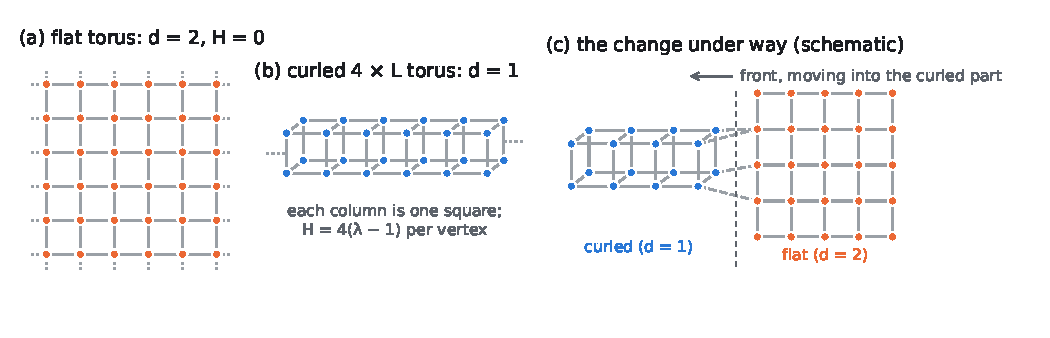
\includegraphics[width=\textwidth]{fig_tori.pdf}
\caption{(a) The flat lattice torus. (b) The $4\times L$ torus drawn as a tube: its short direction is a single
square, so the edges round each column carry three squares. (c) Schematic of the change of Sec.~III, not a
simulation snapshot: the curled order on one side of a single front, the flat order on the other. Spherical
cows being unavailable, every space in this paper is a torus; still, like cows, they burp.}
\label{fig:tori}
\end{figure*}

\emph{Metastability window.} Enumerating every valid graph at $N = 18$ (26 classes up to relabelling)
\cite{repo}, states above the ground state from which every single move costs energy exist for
$1 < \lambda < 1.6$, and at neither $\lambda = 1$ nor any $\lambda \ge 1.6$ (steps of 0.05 up to 1.7, coarser
to 30).

\emph{The way out.} The Markov chain swaps one partner each between two vertices of the same side
(an edge switch preserving the bipartition; Metropolis; the hard-core rule is enforced) \cite{repo}.
A proposal draws two edges one after the other, each uniformly from the $2N$ edges (a vertex of one side and
one of its four slots), so there are $4N^2$ equally likely ordered proposals, and the same two edges drawn in
the opposite order give the same switch: every switch is proposed in two ways. A sweep is $2N$ attempts.
From the perfect $4\times L$ torus the cheapest switches are of two kinds, counted exactly:
move A ($\Delta S = -2$, $\Delta X = -4$; cost $32 - 16\lambda$; $3N$ distinct switches, hence $6N$ ordered
proposals) and move B ($\Delta S = -4$, $\Delta X = -10$; cost $64 - 40\lambda$; $2N$ switches, $4N$
proposals). Move A is therefore offered $2N \times 6N/4N^2 = 3$ times per sweep and B twice, independent of
$N$. Switches that change neither $S$ nor $X$ ($N/2$ of them) do not leave this energy: each reconnects two
neighbouring columns at opposite points, a reflection of the square that twists the torus globally but leaves
every neighbourhood as it was, and every arrangement met along a 60-step walk of such switches (three classes
up to relabelling) has the same counts of A and B \cite{repo}. The mean time to the first exit is therefore an
Arrhenius law whose attempt frequencies are counted, not fitted,
\begin{equation}
\tau(\lambda, g) = \bigl[3 e^{-(32 - 16\lambda)/g} + 2 e^{-(64-40\lambda)/g}\bigr]^{-1},
\label{eq:tau}
\end{equation}
with A the cheaper for $\lambda < 4/3$. Every other exit costs at least 10 more than the cheaper of A and B
for $1.05 \le \lambda \le 1.45$, and Eq.~(\ref{eq:tau}) leaves them out. Those that break two distant edges at
once are offered a number of times per sweep that grows in proportion to $N$ (87 at $N = 192$); counted
exactly, they add at most 2\% to the exit rate at $g = 1.5$ for every $\lambda$ and $N$ studied, and 16\% at
the hottest point of Fig.~\ref{fig:data}(a) ($g = 2.5$, $N = 144$), within its error bar.
That Eq.~(\ref{eq:tau}) does not depend on $N$ is a property of the proposal, not of the barrier: the chain
draws its two edges from the whole graph, so any one region is offered a way out about $1/N$ as often per
sweep, and a dynamics that updated every region at its own fixed rate would give a waiting time falling as
$1/N$.

\section{Decay at fixed coupling}

At $\lambda = 1.25$ the minimum energetic barrier to leave the perfect curled torus, the cost of move A, is
$\Delta E^\ddagger = 12$. It is the barrier to the first exit; whether an exit then grows into a front is a
separate question, answered in Sec.~\ref{sec:lambda}. In an exploratory test (the prediction was written into
the run's configuration before it ran, but not pre-registered), over twelve conditions ($g = 1.4$ to 2.5,
$N = 64$ and 144,
16 runs each), the measured mean waiting time against the move-A term of Eq.~(\ref{eq:tau}) has a plain
mean ratio of 0.98 and a weighted mean of $0.88 \pm 0.06$ (standard error), every ratio between 0.71 and 1.62,
over a ninety-fold range of times [Fig.~\ref{fig:data}(a)]. A weighted straight-line fit of $\ln\tau$ against
$1/g$ gives a barrier of $14.4 \pm 1.0$ at $N = 64$ and $12.1 \pm 0.9$ at $N = 144$; over this narrow range of
$1/g$ the fitted barrier and prefactor trade off, which is why the test above uses the counted values of
both.
Including move B lowers the predicted waiting time by 15\% at $g = 1.5$; across $\lambda$, the full
Eq.~(\ref{eq:tau}) describes the measured waits over two decades (Sec.~\ref{sec:lambda}).

The decay itself was pre-registered \cite{repo}: at $\lambda = 1.25$, $g = 1.5$, thirty decays at each of
$N = 64, 96, 144, 192$, and the adjacency read when the conversion fraction first crossed 25, 50 and 75\%.
The predictions were a memoryless waiting time (coefficient of variation between 0.7 and 1.3), at least
80\% of vertices at $d \in \{1,2\}$ at half conversion, and the converted vertices in one piece holding at
least 70\% of them. All three hold at every size and on two independent sets of seeds (Table~\ref{tab:t7}):
under this dynamics the change starts at one place and runs as a single front, with the two orders on either
side of it and almost nothing in between [Fig.~\ref{fig:data}(b)]. The mean waiting time does not fall with
$N$, as the proposal's $N$-independent rate of exits requires (Sec.~II). The same pre-registration listed
$\lambda = 1.5$; there the torus is not metastable at $g = 1.5$ (its number of squares per vertex falls to 0.95,
below the flat torus's 1, within 50 sweeps in every replica), and no verdict was applied. A separate
pre-registered test of whether a coarse law of a single front governs these decays (T12 in Ref.~\cite{repo};
64 decays at $g = 1.5$ and 2.0, under Metropolis and Glauber acceptance) came out NOT ESTABLISHED: 21 of the 59
that nucleated converted in more than one patch, mostly at the warmer coupling, and the front's rate fell roughly
as $N^{-0.7}$.

The coefficient of variation is a coarse test of memorylessness. Checked afterwards and not pre-registered,
the whole distribution is exponential too [Fig.~\ref{fig:data}(c)]: pooled over conditions after dividing each
time by its condition's mean, the 432 first exits we recorded give a Kolmogorov--Smirnov distance
$D = 0.035$ from the unit exponential ($p = 0.53$), and the 240 of them counted move by move
(Sec.~\ref{sec:lambda}) are exponential with the mean of Eq.~(\ref{eq:tau}) itself, nothing estimated
($p = 0.85$). The pre-registered waits pass once a detection artefact of the protocol is allowed for, and one
feature of the far tail at $\lambda = 1.05$ is unexplained; both are described in Methods.

\begin{table}[b]
\caption{The decay of the $4\times L$ torus at $\lambda = 1.25$, $g = 1.5$ (first run / independent rerun,
thirty decays each).}
\label{tab:t7}
\begin{ruledtabular}
\begin{tabular}{lcccc}
$N$ & mean wait & CV & $d \in \{1,2\}$ at 50\% & largest piece \\
\hline
64  & 871 / 660  & 0.91 / 0.84 & 0.990 / 0.998 & 0.98 / 0.99 \\
96  & 913 / 928  & 1.10 / 1.02 & 0.990 / 0.988 & 0.95 / 0.96 \\
144 & 856 / 743  & 1.01 / 0.76 & 0.997 / 0.997 & 0.92 / 0.96 \\
192 & 1039 / 1428 & 0.87 / 1.19 & 0.995 / 0.995 & 0.85 / 0.92 \\
\end{tabular}
\end{ruledtabular}
\end{table}

\begin{figure*}
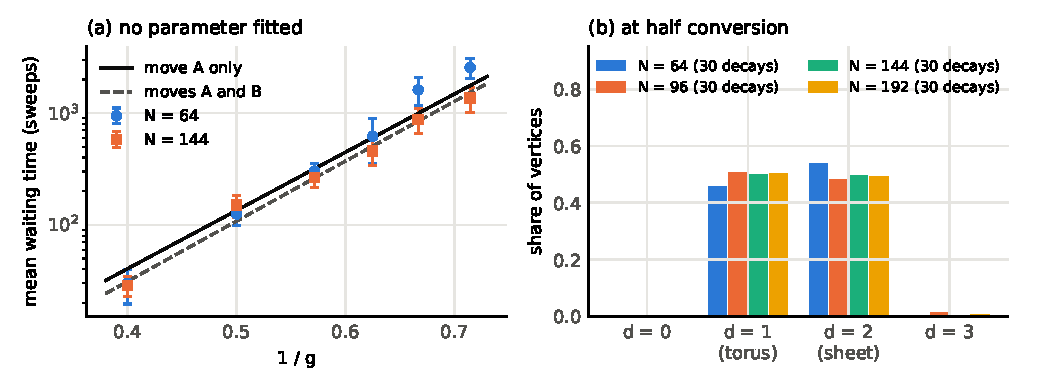
\includegraphics[width=\textwidth]{fig1.pdf}
\caption{(a) Mean waiting time of the perfect $4\times L$ torus at $\lambda = 1.25$ against inverse coupling,
sixteen runs per point; error bars are one standard error of the mean. Lines: Eq.~(\ref{eq:tau}) using move A
only (solid) and moves A and B (dashed); nothing is fitted. (b) Share of vertices at each local dimension $d$
when half the torus has converted, averaged over the thirty decays per size of the rerun in
Table~\ref{tab:t7}. (c) Share of tori still waiting against time in units of the mean of its condition,
pooled, on a logarithmic scale; the dashed line is the exponential $e^{-x}$ of a memoryless wait. Blue: all
432 recorded first exits (twelve conditions of panel a, and six cells of the count in Sec.~\ref{sec:lambda}).
Orange: the 589 decay waits of the $\lambda$ map beyond the 200-sweep watch, for tori not yet changing when
the watch ended (Methods). Not pre-registered.}
\label{fig:data}
\end{figure*}

The energy released is exact. After the burp, 24 to 28 of 30 decays per size rest on the flat torus with
release $\varepsilon$ per vertex to within 1\%. The others settle on defected sheets, read from their wiring:
most often combinations of small defects of 8 to 45 units, and less often the four-point relic of Sec.~IV, a
closed loop of four vertices at $d = 1$ with $S = N + 1$ and, in its commonest form, $X = 6$, costing
$24\lambda - 16$ (14 at $\lambda = 1.25$). Whether these states are stable or only slow is not known. The
pre-registered verdict, a two-state change, holds at $N = 64$, 96 and 192, under an energy gate the author
amended four times: once after the first runs, to fix when the release is read, and three times after the rerun
whose verdict each amendment bore on (to allow the four-point relic, to replay the decays that reached the settle
cap, and to read unusual resting states from their wiring); every amendment is on the record with its timing
\cite{repo}. The three predictions, which concern the first switch, were not amended and held on both sets of
seeds. At $N = 144$ one decay changed state inside its final measuring window and the size was set aside by the
energy gate as written, with all three predictions holding there too.

For contrast: at the same $\lambda = 1.25$ the change out of the random phase shows one hump in the
energy distribution at every coupling, size and replica we ran, with any latent heat below 1.28 per vertex
at $N = 100$ and falling with $N$ \cite{repo}; the pre-registered verdict there is INCONCLUSIVE, because one of
its criteria cannot be read where the cold phase sits at zero energy and the replacement adopted for it reads the
edge of the scan rather than the transition. At this $\lambda$ the sharp change is between orders.

\section{Sealed system}

To follow the released energy we replace the heat bath by Creutz demons \cite{Creutz83}, which makes the
simulation microcanonical: $C$ stores, each
never negative; each attempted move picks one store to pay for it or be paid, and is refused if that store
cannot pay. $H$ plus the stores' contents is conserved exactly, checked to the last unit in every run, and
the stores' mean reads the temperature. This is one energy-conserving version of the same local dynamics, not
the unique dynamics of a sealed system, and what follows is about it.

\emph{A local, size-independent threshold (exploratory).} With one store holding a seed $s$ and nothing else,
the torus
converted in 8 of 8 runs for $s \ge 12$ and in 0 of 8 for $s \le 11.5$ (seeds 4 to 16), at each of
$N = 48, 64, 96, 144, 192$ (320 runs). Twelve is $\Delta E^\ddagger$, the cost of move A. With nothing to
spare the torus never converts, although the flat torus is lower. That nothing below 12 can set it off, from the
perfect torus and from the twisted arrangements met by the walk of Sec.~II, holds for any energy-conserving dynamics made of
single switches, since no switch out of them costs less; that 12 always
sufficed is a property of this one. The activation energy is fixed while the release, $\varepsilon N$, grows
with the system.

\emph{The reservoir must absorb the release.} With the seed in one of $C$ stores, $C$ setting the reservoir's
heat capacity ($N = 64, 96, 192$; twenty runs each; 420 runs): the converted region melts into the random
phase in 17 to 20 of 20 runs for $C \le N/16$ and in 9 to 16 of 20 at $C = N/8$; at $C = N/4$ most runs
end partly converted or partly melted; for $C \ge N/2$ the flat torus results in 18 to 20 of 20. The crossover scales with $N$, as a release of $\varepsilon N$ into $C$
stores against a melting coupling near 3.5 predicts ($C^* \approx N/3.5$). No run stalled with both orders
present and the bath below the melting coupling: under this protocol we find no evidence of a temperature at
which the curled and flat tori coexist.

\emph{About one relic at every size.} In the coldest box ($C = 2N$), the number of relic defects per
converted torus is $0.90 \pm 0.31$, $0.85 \pm 0.37$, $1.05 \pm 0.22$ and $0.95 \pm 0.22$ at
$N = 64, 96, 192, 288$ (mean $\pm$ standard deviation over twenty runs each; a weighted fit against $N$ gives
a slope of $0.0003 \pm 0.0003$ per vertex, standard error). The defect is the four-point loop above (14 units),
its points spanning one to four of the torus's original columns and lying along the torus, or occasionally a
two-vertex twist (20 units). So the count is of order one, with no measurable growth, across the
sizes we could reach. We find no dependence of where the relic sits on where the change started: the pre-registered
test of whether it sits opposite the start or at it finds neither \cite{repo}, and, checked afterwards, a
randomisation test that rotates each relic through every column of its torus with the start held fixed places
the observed mean distance at $p = 0.67$ and $0.59$ ($N = 64$ and 96; 36 and 28 runs with one relic).

\section{Dependence on \texorpdfstring{$\boldsymbol{\lambda}$}{lambda}}
\label{sec:lambda}

The decay was mapped at $\lambda = 1.05$ to 1.45 in steps of 0.05, with the protocol of Sec.~III at all four
sizes and thirty decays per ($\lambda$, $N$) (Table~\ref{tab:lambda}, Fig.~\ref{fig:lambda}). The torus counts as
stuck at ($\lambda$, $N$) when more than half its decays are still at least 75\% torus after the 200-sweep rest
that defines the waiting time (the pre-registered definition, PREREGISTRATION T8 in Ref.~\cite{repo}).

The torus is stuck from $\lambda = 1.05$ to 1.35 at every size and not at 1.40 or 1.45; Eq.~(\ref{eq:tau}) puts
the mean wait at 200 sweeps at $\lambda = 1.345$, just above $4/3$, where move B takes over. Wherever it is stuck, the change keeps the character of
Sec.~III: at half conversion 95 to 100\% of vertices belong to one order or the other, the converted region is
one piece holding 76 to 100\% of it, and the release is exactly $\varepsilon$ per vertex wherever the flat
torus is reached. The mean waiting time follows Eq.~(\ref{eq:tau}) with nothing fitted over two decades
[Fig.~\ref{fig:lambda}(a)], and departs from it at both ends for different reasons. Near the edge the departure
is in the measurement: a wait cannot be recorded before the 200-sweep watch ends (first check at 205), and for
waits spread exponentially with mean $\tau$ the expected recorded mean is about $205 + \tau e^{-205/\tau}$
(dashed; also fitted to nothing): 462 at $\lambda = 1.30$ and 265 at 1.35, against 403--505 and 280--350
measured. Near $\lambda = 1$ the measured waits run 15 to 43\% longer than Eq.~(\ref{eq:tau}), 1 to 1.4
standard errors per cell. A direct test does not reproduce this (PREREGISTRATION T22 in Ref.~\cite{repo}):
counting every accepted move in forty further decays per cell at $\lambda = 1.05$, 1.10 and 1.25 and $N = 64$
and 96, the first exit arrives when Eq.~(\ref{eq:tau}) says, within one standard error in all six cells, and
its distribution is exponential with that mean (Sec.~III). The same count separates the barrier from the rest
of nucleation. $\Delta E^\ddagger$ is the barrier to the first exit; about a third of exits then return to the
torus instead of growing into a front, a transmission coefficient $\kappa = 0.56$ to 0.68 in the language of
transition-state theory, with no trend in $\lambda$. Recrossings add to the time to convert, not to the time to
the first exit, and do not single out small $\lambda$. We read the excess near $\lambda = 1$ as statistical,
with one reservation: at $\lambda = 1.05$ three waits of 200 lie near 80,000 sweeps, which an exponential
makes unlikely (Methods); the one among the map's decays raises its cell's mean from 9629 to 11915, and the
other cells stay 3 to 27\% above Eq.~(\ref{eq:tau}) without their largest wait. How completely the change finishes
depends on $\lambda$ [Fig.~\ref{fig:lambda}(b)]: at $\lambda = 1.05$ every decay ends at the flat torus, while the
share ending on a defected sheet rises to 21\% at 1.30 and 54\% at 1.35. At fixed coupling, then, the relic is
a feature of the larger coefficients, and near $\lambda = 1$ the change is clean. Beyond the edge
($\lambda \ge 1.40$) the change starts more and more often in several places at once (in about half the decays at
$N = 64$ and in all of them at $N = 192$) and ends mostly as a defected sheet.

The pre-registered verdict for the map as a whole is inconclusive, and the reason is stated. Besides the
coexistence and single-front criteria, which hold everywhere the torus is stuck, it required the waiting times to
be memoryless, with a coefficient of variation between 0.7 and 1.3; at thirty decays that band is about two
standard errors wide, and it fails in nine of the 24 stuck cells the map ran (at two sizes at $\lambda = 1.10$,
three at 1.30 and all four at 1.35). At
$\lambda = 1.35$ the energy check also fails for two to five decays per size, whose final states match none of
the allowed ones. A repair computed before being proposed (the variation of the time after the rest) changes no
verdict. Tested afterwards on the whole distribution rather than its coefficient of variation, the waits of the
stuck cells are exponential once the protocol's detection artefact is set aside [Fig.~\ref{fig:data}(c);
Methods].

The map was repeated twice with 120 decays per cell and fresh seeds, each repeat pre-registered with its rules
fixed before it ran \cite{repo}. The first repeat replaced the memoryless band by the central 99.9\% range of the
coefficient of variation of an exponential sample of the same size, applied to the time after the rest; that check
then held in every stuck cell up to $\lambda = 1.25$ and in three of four sizes at 1.30, but the unchanged energy
check failed at every size at 1.30. The reason, read after the fact and not scored, is that it compared a window
average of the energy with the exact energy of the final graph, and the sheet's own thermal excitations at
$g = 1.5$ exceed its 1\% tolerance in a few decays per hundred. The second repeat replaced that check with one that asked only that each
decay's saved final graph exist and be valid, which held in all 28 cells, and read the energy exactly from those
graphs, reporting it rather than gating on it; two orders and one front held in every cell up to 1.30 as before.
The memoryless check now failed in four cells: at $N = 64$ ($\lambda = 1.25$ and 1.30), each on a single wait 24
and 76 times the predicted mean $\tau$, and at $N = 192$ (1.30) and 144 (1.35), with coefficients of variation of
1.53 and 1.41 against a band ending at 1.38. So three runs have tripped three different criteria, on a band, a
catalog, and the spread of the waits, while the physics has read the same each time.
The break-up at the edge (Sec.~\ref{sec:lambda}) appeared in both repeats: pooled over sizes from $\lambda = 1.30$
to 1.35, the share of decays ending at the flat torus falls from 0.71 to 0.47 and from 0.74 to 0.49, and the share
whose converted region is in several pieces at a quarter conversion rises from 0.44 to 0.69 and from 0.43 to 0.68.
The rare very long wait, first seen at $\lambda = 1.05$ (Methods), is now on the record at 1.25 and 1.30 as well,
always at the smaller sizes; it is a feature to study on the saved graphs, not a rule to rewrite after the fact.

\begin{table}[b]
\caption{The map along $\lambda$ at $g = 1.5$ (ranges over $N = 64$ to 192; thirty decays per cell; $\lambda = 1.25$
from the two runs of Table~\ref{tab:t7}, not rerun in the map, its flat share from the second). Two orders: share of vertices at $d \in \{1,2\}$ at half conversion. Flat: share of
decays ending at the flat torus.}
\label{tab:lambda}
\begin{ruledtabular}
\begin{tabular}{lcccc}
$\lambda$ & $\tau$, Eq.~(\ref{eq:tau}) & mean wait & two orders & flat \\
\hline
1.05 & 8330 & 9617--11915 & 1.000 & 100\% \\
1.10 & 4844 & 4154--6626 & 0.998--1.000 & 98\% \\
1.15 & 2788 & 2191--3834 & 0.996--0.999 & 97\% \\
1.20 & 1570 & 1132--1716 & 0.996--0.998 & 93\% \\
1.25 & 845 & 660--1428 & 0.988--0.998 & 88\% \\
1.30 & 419 & 403--505 & 0.980--0.984 & 79\% \\
1.35 & 183 & 280--350 & 0.948--0.963 & 46\% \\
1.40 & 68 & not stuck & 0.911--0.924 & 31\% \\
1.45 & 22 & not stuck & 0.799--0.837 & 7\% \\
\end{tabular}
\end{ruledtabular}
\end{table}

\begin{figure*}
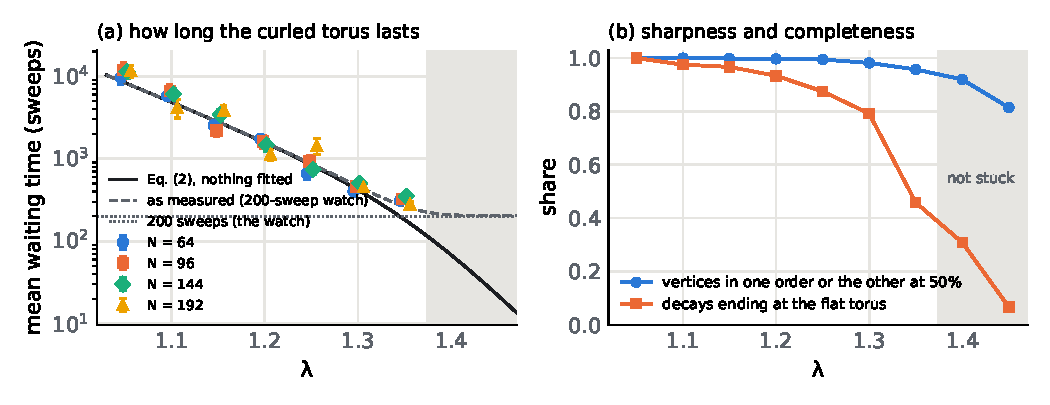
\includegraphics[width=\textwidth]{fig_lambda.pdf}
\caption{The map along $\lambda$ at $g = 1.5$. (a) Mean waiting time where the torus is stuck, four sizes, thirty
decays each; error bars are one standard error of the mean. Lines:
Eq.~(\ref{eq:tau}) (solid) and the same prediction as it would be recorded given the 200-sweep watch,
$205 + \tau e^{-205/\tau}$ (dashed); both fitted to nothing. Shaded, the $\lambda$ at which it is not stuck.
(b) Share of vertices in one order or the other at half conversion, and share of decays ending at the flat
torus, pooled over sizes.}
\label{fig:lambda}
\end{figure*}

\section{Discussion}

At $\lambda = 1$, which is CQG, the flat, curled and 4-cube tori are degenerate and the change
releases nothing. The burp described here therefore belongs to the family on the $\lambda > 1$ side; the map of
Sec.~\ref{sec:lambda} shows it keeping its character down to $\lambda = 1.05$, where it is cleanest, with a
release $\varepsilon = 4(\lambda - 1)$ that vanishes at the CQG value. The same
questions can be asked in CQG itself, at $\lambda = 1$, of regions stuck in a different discrete arrangement
inside a curved background \cite{T24}, such as the allotrope of Ref.~\cite{T25} (Fig.~9): whether such a region is metastable, and whether it gives way by a front with a
definite release. The tools used here (exact barrier counting, front tracking, sealed baths) apply
unchanged.

What has been shown, stated with its dynamics: an ordered, curled torus sits a known energy per vertex above
the flat one; under local switch dynamics it escapes over a single move whose cost, $\Delta E^\ddagger$, does
not depend on size; after escape the conversion runs as a sharp front between the two orders; and under an
energy-conserving version of the same dynamics a fixed local activation unlocks a release that grows with the
system. The energies hold for any dynamics made of these switches. The rates, and with them the waiting
times, their independence of $N$ and the transmission coefficient, are properties of this chain.

\emph{Labelled or interchangeable vertices.} All runs here, like the published CQG simulations we know of
\cite{KTB19,T25}, treat vertices as labelled: two graphs that differ only by renaming vertices are different
states. Treating vertices as interchangeable, as identical particles are, counts each unlabelled graph once
\cite{DQM25}; on labelled graphs this weights every state by its number of symmetries (the order of its
side-preserving automorphism group), and a chain samples it by multiplying each acceptance by the ratio of
the two counts. The choice leaves every energy unchanged, and so the gap $\varepsilon$, the barrier
$\Delta E^\ddagger$, the existence of the one-move path and the least seed a sealed system needs. It changes
the rates. The perfect curled torus has $2N$ symmetries, the twisted arrangements it reaches without leaving
its energy have $N$ or $2N$, and every arrangement one move A away has 2 (counted exactly at $N = 64$ and
96 \cite{repo}), so each exit would be accepted $N/2$ to $N$ times less often: the escape would be slower by a
factor of order $N$, and the waiting time would grow with the system instead of staying flat. This is
transition-state reasoning: the choice fixes the equilibrium weights but not the kinetics, so ``of order $N$'' is
the change in the effective barrier, not a derived clock. We have not run the decay with interchangeable vertices.

Not claimed: that this chain is the physical time evolution of anything; a first-order transition in the
thermodynamic sense (this is the decay of a metastable state at fixed coupling, and ``sharp'' is used in the
pre-registered sense above); anything at sizes beyond 288; why the cold box leaves about one defect.

\emph{Outlook (motivation, not a result).} This work is motivated by the hypothesis that space emerged from a
specific ordered precursor through a sharp change of this kind, a lattice cousin of false-vacuum decay
\cite{C77}, releasing a definite energy and leaving relics behind. Nothing here tests that hypothesis beyond
showing that a graph energy one coefficient away from a model of emergent geometry contains such a change. We note only that the relic found here, of
fixed size and about one per change at every size we reached, is the kind of object a dark-matter relic of such a
change would have to be, though it anneals away at every fixed coupling we tried, survives when the box cools
faster than it heals, and grows in number with the number of seeds that start the change \cite{repo}; and that the
change
needs a push of fixed size while what it releases grows with the system.

\section*{Methods and data}

Simulations use single-edge switches that preserve the bipartition, with Metropolis acceptance; the chain
reproduces exact averages computed by enumerating every valid graph at $N = 16$ and 18, and the published
square density of Ref.~\cite{KTB19} (Fig.~8a) at $N = 160$ to rms 0.005; it does not reproduce the steeper
curve of Ref.~\cite{T25} (Fig.~3) at the same size, from which it differs by up to 0.41 between $g = 2$ and 6.3, a
disagreement between the two published figures that is still open. Every kinetic quantity quoted is
for this chain (Introduction). Seeds are fixed in configuration
files; every result file carries its configuration and software versions. Predictions and analysis rules
were committed before the runs they concern, with every amendment recorded. Code, data, configurations and
pre-registrations: \cite{repo}.

\emph{Checks added after the runs} (not pre-registered; suggested by an AI-generated review, see Acknowledgments; committed data, no new
simulation \cite{repo}). To test whether waits are exponential, each time is divided by the mean of its
condition and the pooled times are compared with the unit exponential by the Kolmogorov--Smirnov distance
$D$. Because the means come from the same data, $p$ is from a parametric bootstrap that repeats the whole
procedure: 10,000 simulated data sets with each condition's mean and count, recorded as the runner records
them. The 432 first exits (twelve conditions of Fig.~\ref{fig:data}(a), recorded to the sweep, and six cells
of Sec.~\ref{sec:lambda}, to the attempt) give $D = 0.035$, $p = 0.53$; taken singly, two of the eighteen
conditions give $p < 0.05$, both at $\lambda = 1.05$ (see below). The pre-registered waits of Secs.~III
and~\ref{sec:lambda} are read every five sweeps and only after the 200-sweep watch, so we test the time beyond
the first check, which for a memoryless wait is again exponential with the same mean. A torus that begins to
change during the watch widens the resting spread that sets the detection threshold, so it is detected late,
just after the watch. The map records how far each torus had converted at sweep 200; the 589 waits of its
stuck cells from tori not yet changing then give $D = 0.030$, $p = 0.55$, against $p = 0.03$ for all 865
waits of Secs.~III and~\ref{sec:lambda} with nothing set aside. Table~\ref{tab:t7}'s waits predate that record;
for them the deviation fades as the clock is started later, $p < 10^{-3}$, 0.012, 0.094 and 0.66 from sweeps
205, 255, 305 and 405, as an artefact confined to the start of the wait would. One feature is not explained:
at $\lambda = 1.05$, three of 200 waits (the 80 first exits of Sec.~\ref{sec:lambda} and the 120 decays of
the map) exceed 75,000 sweeps, where exponentials with the measured means give 0.19 such waits, and three or
more with probability $10^{-3}$. Whether this is chance, or something we have not identified that slows some
runs, is open.
The exit counts behind Eq.~(\ref{eq:tau}), the twisted arrangements at the torus's energy and their symmetry
counts are enumerated exactly, with no simulation \cite{repo}.

\section*{Changes from the first version}

A referee-style reading of the first version, generated with Claude (Anthropic) and checked point by point
against the record and the committed data \cite{repo}, found the following, all corrected here; no result was
removed and no verdict changed. The first version said every verdict quoted was pre-registered; two results it
quoted, the Arrhenius test of the waiting time and the 12-unit seed threshold, were exploratory, and are now
labeled so. The two-state verdict at $\lambda = 1.25$ was reached after four amendments to its energy gate, three
written after the data they judged; this is now stated in the abstract and Sec.~III. ``Memoryless'' is now ``close
to memoryless'', with the failing checks named, and the abstract's summary of the $\lambda$ map now says that all
three runs were inconclusive by the letter and that the single front begins to break up at $\lambda = 1.35$.
Corrected counts and descriptions: the memoryless check of the map failed in nine of 24 stuck cells, not five of
28; the second repeat's gate asked only for a complete, valid record of final graphs, and of its four memoryless
failures two are single very long waits at $N = 64$ and two are wide spreads; beyond the edge the change starts in
several places in a stated share of decays, rather than ``everywhere at once''; Eq.~(\ref{eq:tau}) crosses 200
sweeps at $\lambda = 1.345$, not 1.33; Table~\ref{tab:lambda} gains its $\lambda = 1.25$ row. The commonest
resting state after the burp is a combination of small defects, not the four-point relic, and the relic is a
closed loop of four whose points lie along the torus, rather than always one curled column. For $\lambda > 1$ the
ground state is a family, the flat torus and its twisted relatives, not unique, and the twisted family was checked
along a walk, not exhaustively. The Metropolis acceptance and the ordered-pair proposal are our choices, not the published
sampler's. Added caveats: the coarse front law (T12) was not established; at $\lambda = 1.5$ the torus is not
metastable; the chain does not reproduce Ref.~\cite{T25} Fig.~3; the random-phase verdict at $\lambda = 1.25$ is
inconclusive; the interchangeable-vertex estimate is transition-state reasoning; the relic anneals at fixed
coupling and its number grows with the number of seeds; and ``stuck'' is the pre-registered definition.

\begin{acknowledgments}
Code, analysis and text were drafted with Claude (Anthropic), directed and checked by the author; every
kernel is tested against an independent computation before use. A review of an earlier draft generated with
ChatGPT (OpenAI) prompted the checks marked as added after the runs, and several clarifications. We thank
C.~A.~Trugenberger for correspondence.
\end{acknowledgments}

\begin{thebibliography}{99}
\bibitem{T17} C.~A. Trugenberger, J. High Energy Phys. \textbf{09} (2017) 045, arXiv:1610.05934.
\bibitem{KTB19} C.~Kelly, C.~A. Trugenberger, and F.~Biancalana, Class. Quantum Grav. \textbf{36}, 125012 (2019), arXiv:1901.09870.
\bibitem{T25} C.~A. Trugenberger, \emph{Networks as the fundamental constituents of the universe}, arXiv:2512.17676.
\bibitem{GV21} A.~Gorsky and O.~Valba, Phys. Rev. D \textbf{103}, 106013 (2021), arXiv:2101.04072.
\bibitem{T24} C.~A. Trugenberger, \emph{Dark matter and dark energy in combinatorial quantum gravity}, arXiv:2409.09385.
\bibitem{Creutz83} M.~Creutz, Phys. Rev. Lett. \textbf{50}, 1411 (1983).
\bibitem{DQM25} K.~Betre and N.~Lewis, \emph{Dynamical quantum multigraphs}, arXiv:2509.08296 (2025).
\bibitem{C77} S.~Coleman, Phys. Rev. D \textbf{15}, 2929 (1977).
\bibitem{repo} E.~Smith, RecreationalPhysics, \url{https://github.com/EmilySmithCreate/RecreationalPhysics}.
\end{thebibliography}

\end{document}
